%% Cric losange — dessin d'ensemble simplifié, pièces numérotées (0 à 9).
\documentclass[tikz,border=4pt]{standalone}
\usepackage{liaisons}
%% Dessin d'ensemble simplifié du cric losange (cric de voiture à vis), vu dans le plan (x, y).
%% Inclus par mecanisme-cric-losange-dessin.tex et mecanisme-cric-losange-classes.tex, qui définissent
%% \piece{N}{chemin} (surface d'une pièce : hachurée dans le dessin, colorée dans la vue « classes »),
%% \trait{N}{chemin} (trait fin de la même pièce : pli de tôle, filet de la vis) et \criclabels.
%% Cotes en cm, θ = 35° : O = (0 ; 0) ; L = (−1,311 ; 0,918) ; R = (1,311 ; 0,918) ; T = (0 ; 1,836).
%% Les quatre barres du losange ont la même longueur : 1,6 cm entre axes.
\newcommand\cric{%
  \begin{scope}[line width=0.6pt, line join=round]
    % --- le sol (le cric y est simplement posé)
    \draw[line width=0.5pt, black!60] (-2.10,-0.34) -- (2.10,-0.34);
    \foreach \sx in {-2.00,-1.80,...,2.05} {\draw[line width=0.4pt, black!60] (\sx,-0.34) -- ({\sx-0.16},-0.52);}
    % --- 0 : socle posé au sol, avec sa chape pour le pivot inférieur O
    \piece{0}{(-1.05,-0.34) -- (1.05,-0.34) -- (0.86,-0.08) -- (-0.86,-0.08) -- cycle}
    \piece{0}{(-0.26,-0.08) rectangle (0.26,0.22)}
    % --- 1 et 2 : barres inférieures (barres plates, dessinées dans leur repère : origine O)
    \begin{scope}[shift={(0,0)}, rotate=145]     % 1 : vers L
      \piece{1}{(-0.17,-0.115) rectangle (1.77,0.115)}
      \trait{1}{(-0.17,0.050) -- (1.77,0.050)}
    \end{scope}
    \begin{scope}[shift={(0,0)}, rotate=35]      % 2 : vers R
      \piece{2}{(-0.17,-0.115) rectangle (1.77,0.115)}
      \trait{2}{(-0.17,-0.050) -- (1.77,-0.050)}
    \end{scope}
    % --- 3 et 4 : barres supérieures (origines L et R)
    \begin{scope}[shift={(-1.311,0.918)}, rotate=35]    % 3 : de L vers T
      \piece{3}{(-0.17,-0.115) rectangle (1.77,0.115)}
      \trait{3}{(-0.17,0.050) -- (1.77,0.050)}
    \end{scope}
    \begin{scope}[shift={(1.311,0.918)}, rotate=145]    % 4 : de R vers T
      \piece{4}{(-0.17,-0.115) rectangle (1.77,0.115)}
      \trait{4}{(-0.17,-0.050) -- (1.77,-0.050)}
    \end{scope}
    % --- 8 : la vis (corps fileté) puis 9 : la manivelle coudée, à droite de R
    \piece{8}{(-1.92,0.863) rectangle (1.98,0.973)}
    \trait{8}{foreach \tx in {-1.85,-1.63,...,1.90} {({\tx},0.863) -- ({\tx+0.09},0.973)}}
    \piece{9}{(1.90,0.850) -- (2.30,0.850) -- (2.30,1.46) -- (2.74,1.46) -- (2.74,1.59)
              -- (2.17,1.59) -- (2.17,0.986) -- (1.90,0.986) -- cycle}
    % --- 6 et 7 : les écrous (celui de gauche a un filet à gauche, celui de droite un filet à droite)
    \piece{6}{(-1.57,0.688) rectangle (-1.05,1.148)}
    \piece{7}{(1.05,0.688) rectangle (1.57,1.148)}
    % --- 5 : plateau d'appui (gorge qui reçoit le bas de caisse) et sa chape en T
    \piece{5}{(-0.24,1.70) rectangle (0.24,1.90)}
    \piece{5}{(-0.62,1.90) -- (0.62,1.90) -- (0.62,2.14) -- (0.34,2.14) -- (0.34,2.00)
              -- (-0.34,2.00) -- (-0.34,2.14) -- (-0.62,2.14) -- cycle}
    % --- amorce du bas de caisse de la voiture (ce n'est pas une pièce du cric)
    \draw[line width=0.5pt, fill=black!8] (-1.25,2.14) -- (1.25,2.14) -- (1.25,2.58) -- (-1.25,2.58) -- cycle;
    \node[font=\small, black!65] at (0,2.36) {bas de caisse};
    % --- axes des pivots (petits cercles) et points caractéristiques
    \foreach \pt in {(0,0), (-1.311,0.918), (1.311,0.918), (0,1.836)} {\draw[line width=0.5pt, fill=white] \pt circle (0.075);}
    \foreach \pt in {(0,0), (-1.311,0.918), (1.311,0.918), (0,1.836)} {
      \draw[blue, line width=0.5pt] \pt ++(-0.13,0) -- ++(0.26,0) \pt ++(0,-0.13) -- ++(0,0.26);}
    \node[blue, font=\small, inner sep=1pt] at (0.28,-0.22) {O};
    \node[blue, font=\small, inner sep=1pt] at (-1.44,0.55) {L};
    \node[blue, font=\small, inner sep=1pt] at (1.44,0.55) {R};
    \node[blue, font=\small, inner sep=1pt] at (0.42,1.86) {T};
    \criclabels
  \end{scope}}

\begin{document}
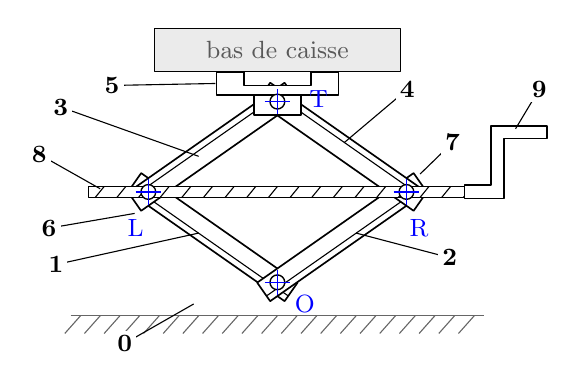
\begin{tikzpicture}[x=1.25cm,y=1.25cm]
% surfaces : seules les pièces « coupées » (socle et écrous, pour montrer le filetage)
% sont hachurées ; les autres sont vues de côté, contour et fond blanc.
\newcommand\vue[1]{\draw[line width=0.6pt, line join=round, fill=white] #1;}
\newcommand\piece[2]{\ifcase#1\relax
  \hachures{#2}%    0 socle
  \or \vue{#2}%     1 barre inférieure gauche
  \or \vue{#2}%     2 barre inférieure droite
  \or \vue{#2}%     3 barre supérieure gauche
  \or \vue{#2}%     4 barre supérieure droite
  \or \vue{#2}%     5 plateau
  \or \hachuresb{#2}%  6 écrou gauche (coupé : on voit le filet)
  \or \hachuresb{#2}%  7 écrou droit
  \or \vue{#2}%     8 vis
  \else \vue{#2}%   9 manivelle
  \fi}
\newcommand\trait[2]{\draw[line width=0.4pt] #2;}
% repères de pièces : numéro dans une pastille blanche, relié à la pièce par un trait fin
\newcommand\criclabels{%
  \foreach \n/\pt/\lab in {0/{(-0.85,-0.22)}/{(-1.55,-0.62)}, 1/{(-0.80,0.50)}/{(-2.25,0.18)},
                           2/{(0.80,0.50)}/{(1.75,0.25)},     3/{(-0.80,1.28)}/{(-2.20,1.78)},
                           4/{(0.68,1.42)}/{(1.32,1.96)},     5/{(-0.63,2.02)}/{(-1.68,2.00)},
                           6/{(-1.45,0.70)}/{(-2.32,0.55)},   7/{(1.45,1.10)}/{(1.78,1.42)},
                           8/{(-1.80,0.95)}/{(-2.42,1.30)},   9/{(2.42,1.56)}/{(2.66,1.96)}} {
    \draw[line width=0.4pt] \lab -- \pt;
    \node[fill=white, inner sep=1.5pt, font=\small\bfseries] at \lab {\n};
  }}
\cric
\repere{(2.15,-0.70)}{x}{y}{1}
\end{tikzpicture}
\end{document}
